% DOCUMENT SETUP ==================================================================================================

\documentclass[a4paper, 12pt]{article}

% PACKAGE IMPORTS =================================================================================================

\usepackage[utf8]{inputenc}    % UTF-8 encoding 
\usepackage{amsmath, amssymb}  % Better equation handling and access to extra math symbols
\usepackage{graphicx}          % Image handling
\usepackage{caption}           % Caption control
\usepackage{subcaption}        % Side by side subfigures
\usepackage{float}             % Precise float placement
\usepackage{geometry}          % A4 paper format
\usepackage{titlesec}          % Section control package
\usepackage{fancyhdr}          % Header and Footer package
\usepackage{longtable}         % Table package
\usepackage{hyperref}
\hypersetup{
    colorlinks=true,       % Enable colored links instead of boxes
    linkcolor=black,       % Section links
    urlcolor=blue,         % URLs
    citecolor=black,       % Citations
}

% PACKAGE SETTINGS ================================================================================================

% Page margin ------------------------
\geometry{margin=1in} % Margin spacing

% Footer and header settings ---------------------------------------------------
\pagestyle{fancy}                   % Page style set to 'fancy'
\fancyhf{}                          % Clears existing header and footer settings
\cfoot{\thepage}

% Section and subsection settings --------------------------------------
\titlespacing*{\section}{0pt}{*3}{*2}  % {left}{before-sep}{after-sep}
\titleformat{\section}[block]          % Formatting option
  {\normalfont\large\bfseries}         % Font style option
  {\thesection .}                      % Section number appearance
  {0.3em}                              % Spacing between number and text
  {}                                   % Section formatting

% META DATA =======================================================================================================

\title{Knight Quest: A Geometric Heuristic Approach to Knight Pathfinding} % Title
\author{Aleksandar Gladović  \\[0.2cm] \href{mailto:alsocial5371@gmail.com}{alsocial5371@gmail.com}}        % Author
\date{July 6, 2025}                 % Date

% DOCUMENT RENDERING ==============================================================================================
\begin{document}

% First page ------------------------------
\maketitle       % Create title
\tableofcontents % Create table of content
\newpage         % Break to new page

% Second page -----------------------------------------------------------------------------------------------------
% Section 1 - Introduction ----------------------------------------------------------------------------------------

\section{Introduction}
This article presents a novel, geometry-inspired solution to the knight’s shortest path problem by exploiting the 
emerging modularity and rotational symmetry of L-shaped knight moves. Rather than relying solely on traditional search 
algorithms, this method models the knight’s movements as base vectors in the complex plane, specifically using the 
canonical vectors (2,1) and (1,2) represented as \( \overrightarrow{u} = 2 + i \) and \( \overrightarrow{v} = 1 + 2i \).
These vectors are then rotated and mirrored according to the signed distance vector between the starting point \( A_{x,y} \)
and the destination \( B_{x,y} \), allowing for a modular decomposition of the knight's path. The solution operates by 
transforming the pathfinding problem into one of rotational alignment and mirrored symmetry, with strategic reference points
\( R_{x,y} \) used to identify optimal paths across different directional regions. By analyzing the periodic structure of 
knight moves—especially across diagonals like \( y = x \) and lines \( y = \frac{x}{2} \) the algorithm leverages the 
repeating alternation in movement patterns to reduce the problem to a combination of sequence evaluation and rotation-based 
projection. The remainder of the article will formalize this model and define its evaluation metrics.

\vspace{1em}
\noindent For Implementation details in python, log files, testing and comparison against BFS check the 
\href{https://github.com/WhyNotAleksandar/knight-quest}{Github repository}.
\newpage

% Third page ------------------------------------------------------------------------------------------------------
% Section 2 - Problem statement -----------------------------------------------------------------------------------

\section{Problem statement}
Find the minimum number of moves for a knight to reach a square on the grid. Optional, construct a path
of knight moves from starting to final square on the grid.

% Section 3 - Reverse path construction ---------------------------------------------------------------------------

\section{Preliminaries}
\vspace{-0.5em}
\begin{figure}[H]
  \centering
  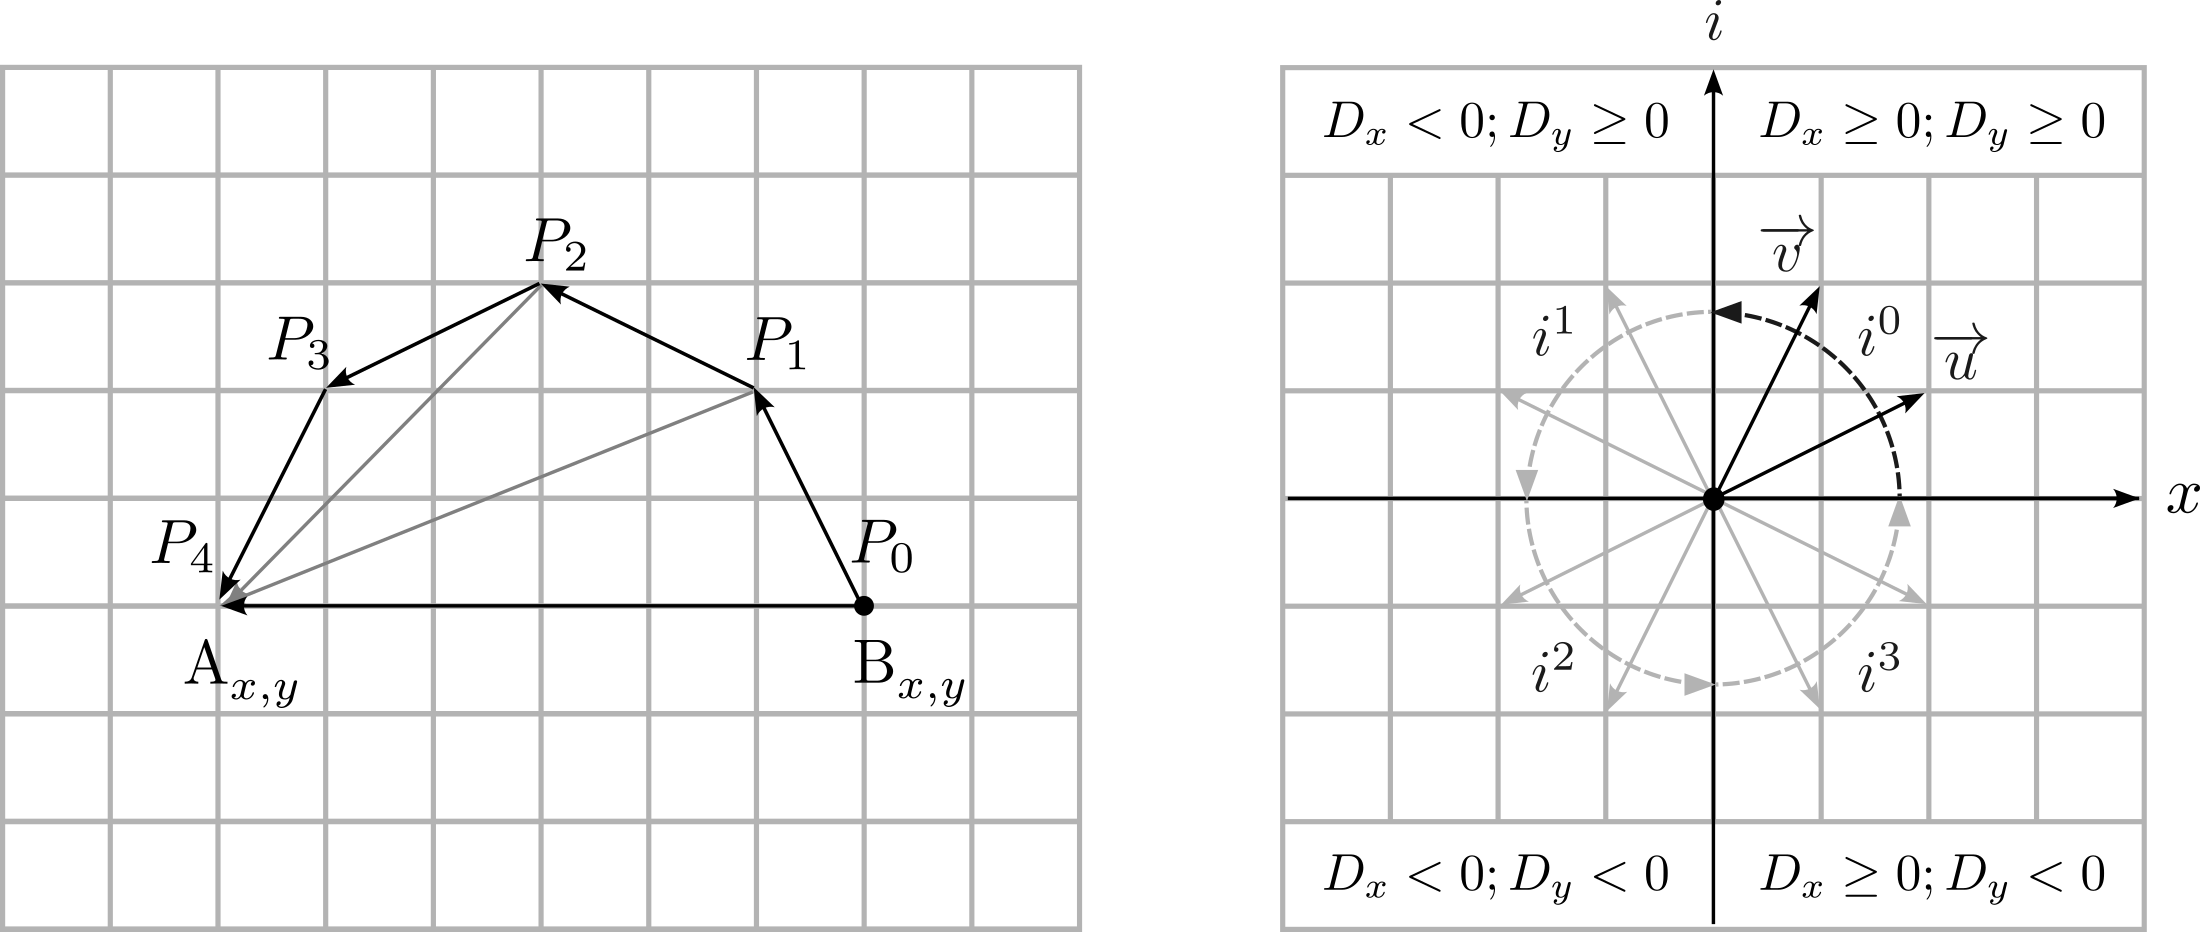
\includegraphics[width=0.9\textwidth]{figures/figure-1.png}
  \caption{Path construction}
\end{figure}

Let: \( A_{x,y} \) be the starting position and \(B_{x,y}\) the final position. \(A_x, B_x\) denotes positions on \(x\)-axis;
\(A_y, B_y\) denotes positions on \(y\)-axis; where \(x,y \in \mathbb{Z}\). \(P_{i,j} = ( p_0, p_1, ... , p_n)\) is a sequence
of path segments where \(0 \le i \le n, j \in \left\{ x, y\right\}\) and \( p_0 = \left\{ B_x, B_y\right\}\). Then
\( f_{seg}(P_i, K)\) is a function that modifies a segment: 
\[
f_{seg}(P_i, K) = \left\{ P_{i,x} + K_x, P_{i,y} + K_y \right\}
\]
Let: \( D_{x,y} \) be the signed distance vector in the \( x \) and \( y \) directions from the path segment \( P_i \)
to the starting position \( A \).
\[
D_{x,y} = f_{dist}(P_i) = \left\{ A_x - P_{i,x}, A_y - P_{i,y} \right\}
\]
Then \( \overrightarrow{u} = 2 + i, \overrightarrow{v} = 1 + 2i \) are knight base vectors in the first quadrant,
where \(u,v \in \mathbb{C}\). \(U_{x,y}\) and \(V_{x,y}\) are real parts of \(90^{\circ}\) counterclockwise rotation 
of those vectors representing knight movement. \(\Delta\theta\) is the rotation scalar of the \(90^{\circ}\) angle 
respectively of \(D\).  \\
\[
U = f_{rot}(u, \Delta\theta) = \left\{ \Re(u \cdot i^{\Delta\theta}), \Im(u \cdot i^{\Delta\theta}) \right\}
\]
\vspace{-1em}
\[
V = f_{rot}(v, \Delta\theta) = \left\{ \Re(v \cdot i^{\Delta\theta}), \Im(v \cdot i^{\Delta\theta}) \right\}
\]
\begin{center}
Quadrant rotations and adjacent square adjustment
\end{center}
\vspace{0.5em}
\[
\Delta \theta =
\begin{vmatrix}
\ 0 & \text{ if }D_{x} \ge 0 \text{ and } & D_{y} \ge 0 \ \\
\ 3 & \text{ if }D_{x} \ge 0 \text{ and } & D_{y} < 0   \ \\
\ 1 & \text{ if }D_{x} < 0   \text{ and } & D_{y} \ge 0 \ \\
\ 2 & \text{ if }D_{x} < 0   \text{ and } & D_{y} < 0   \ 
\end{vmatrix}
\hspace{1em}
|D_{x,y}| = 1 \to \Delta\theta = \Delta\theta + 1
\]
\newpage

% Fourth page -----------------------------------------------------------------------------------------------------
% Section 4 - Reference point -------------------------------------------------------------------------------------

\section{Reference point}
\begin{figure}[H]
  \centering
  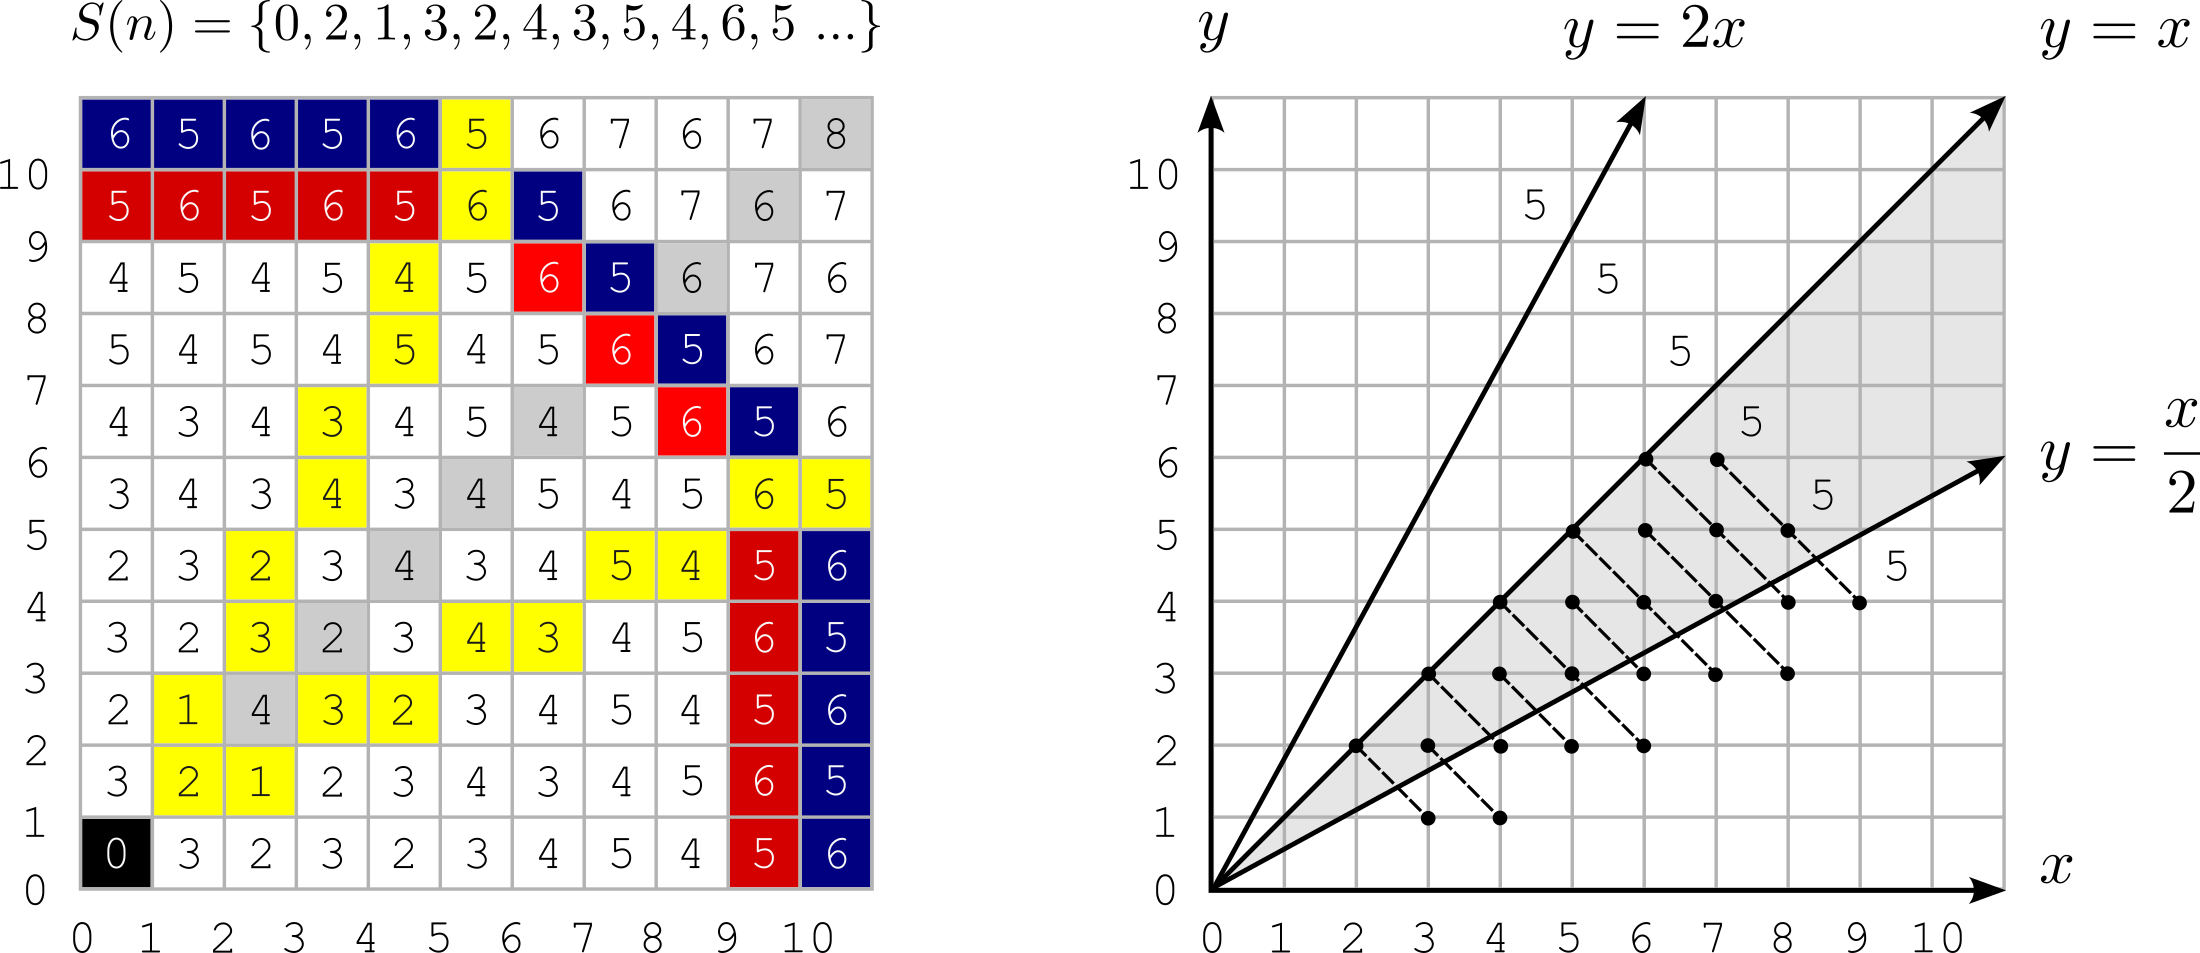
\includegraphics[width=0.9\textwidth]{figures/figure-2.png}
  \caption{Reference point projection}
\end{figure}
Knight moves are mirrored across the main diagonals: \( y = x, y = -x, -y = x \) and \( -y = -x \). They exhibit 
repeating patterns along perpendicular lines, such as from \( y = x \) to \( y = \frac{x}{2} \) or \( y = 2x \), 
where the movement alternates either vertically ( \( x \) to \( y = \frac{x}{2} \) ) or horizontally ( \( y  \) 
to \( y = 2x \) ). By analyzing sequences of moves along the \( y = \frac{x}{2} \) line,  we can determine the 
minimum number of moves required to reach a target square.

\vspace{1em}
\noindent Let \( R_{x,y} \) be a reference point between \( P_i \) and \( A \), independent of orientation or 
direction, due to the mirroring property of knight movement.
\[ 
R_{x,y} = f_{ref}(D) = \left\{ \text{max}(|D_x|,|D_y|), \text{min}(|D_x|,|D_y|) \right\} 
\]

\noindent To determine the minimum number of moves to reach this point, if it lies within the region between
\( y = x \) and \( y = \frac{x}{2} \), we project it into the region below \( y = \frac{x}{2} \) by determining how far 
it must be moved diagonally. Such that:

\vspace{0.5em}
\[
y - \Delta \le \left\lfloor \dfrac{x+\Delta}{2} \right\rfloor \hspace{0.5em} \text{for} \hspace{0.5em} \Delta \in \mathbb{N}
\]
\vspace{0.5em}
\[
y - \Delta \le \dfrac{x + \Delta}{2} \Rightarrow
2y - 2\Delta \le x + \Delta \Rightarrow
2y - x \le 3\Delta \Rightarrow
\Delta \ge \dfrac{2y - x}{3}
\]
\vspace{0.5em}
\[
\text{For first integer this is true: } \Delta = \left\lceil \dfrac{2y-x}{3}\right\rceil
\]
\begin{center}
Then to project the reference point \( R \) into the region of space bellow \( y=\frac{x}{2} \):
\end{center}
\[
R^{'}_{x,y} = \left\{ R_x + \Delta , R_y - \Delta \right\}
\]
\newpage
% Fifth page ------------------------------------------------------------------------------------------------------
% Section 5 - Evaluation function ---------------------------------------------------------------------------------

\section{Evaluation function}
Let \( n \) be the index of the sequence of moves along the line \( y = \frac{x}{2} \), and let \( m \) be the index of the 
sequence of moves along the \( y \)-axis. Then, we can define $n$ and $m$ in terms of the reference point \( R \) 
and its projection:

\vspace{1em}
\[
n,m = f_{term}(R) = \left\{
\begin{array}{l l l}
n = R_x; & m = \left\lceil \frac{n}{2} \right\rceil - R_y; & R_y < \frac{R_x}{2} \\[3pt]
n = R_x^{'}; & m = \left\lceil \frac{n}{2} \right\rceil - R_y^{'};& R_y \ge \frac{R_x}{2} \\[3pt]
n = 5; & m = 0; & R_x = R_y = 2
\end{array}
\right\}
\]

\vspace{1em}
\noindent Let \( S_1(n) = (s_0, s_1, \dots, s_n) \) be a sequence of moves along the line \( y = \frac{x}{2} \). 
Let \( S_2(n, m) = (s_0, s_1, \dots, s_n) \) be the alternating sequence derived from the values of \( S_1(n) \), 
where \( s_n \in \mathbb{W} \). Let \( p(a) \) be a parity function. Then, we define the sequence values as follows: 

\vspace{0.5em}
\[
p(a) = a \bmod 2 \hspace{1.5em}
S_1(n) = \dfrac{n + 3p(n)}{2}
\]
\vspace{0.5em}
\[
S_2(n,m) = S(n) - [ \ p(n) \cdot p(m) \ ] + [ \ p(n-1) \cdot p(m) \ ]
\]

\vspace{1em}
\noindent Therefore, to find the minimum number of moves for a knight to reach a square on the board based on the 
\(n, m \) terms we define the evaluation function as:
\vspace{0.8em}
\[
f_{eval}(n,m) = \left\{
\begin{array}{c l}
S_2(n,m) & n,m > 0 \\[3pt] 
3 & n = m = 1
\end{array}
\right\}
\]
\newpage

% Sixth page ------------------------------------------------------------------------------------------------------
% Section 6 - Solution --------------------------------------------------------------------------------------------

\section{Solution}
To evaluate the moves and construct a path calculate the initial \( D, R \) and \( n, m \):
\[
D = f_{dist}(P_0) \hspace{1em} R = f_{ref}(D) \hspace{1em} n,m = f_{term}(R)
\]
\( f_{eval}(n,m) \) finds the minimum number of moves to reach a square on the board:

\vspace{0.6em}
\[
f_{eval}(n,m) = \left\{
\begin{array}{c l}
S_2(n,m) & n,m > 0 \\[3pt]
3 & n = m = 1
\end{array}
\right\}
\]

\vspace{0.6em}
\noindent \( f_{move}(D) \) applies a move based on the distance and direction to the target square:
\vspace{0.6em}
\[
f_{move}(D) = \left\{
\begin{array}{l l}
D; & \text{max}(D_x,D_y) \ / \ \text{min}(D_x,D_y) = 2 \\[3pt]
U; & f_{eval}(n,m) - f_{eval}(f_{term}(f_{ref}(R_x - 2, R_y - 1))) = 1 \\[3pt]
V; & f_{eval}(n,m) - f_{eval}(f_{term}(f_{ref}(R_x - 1, R_y - 2))) = 1
\end{array}
\right\}
\]

\vspace{0.6em}
\noindent \( f_{path}(P) \) recursively constructs a path from a sequence of valid path segments:
\vspace{0.6em}
\[
f_{path}(P) = f_{path}(P \cup f_{seg}(P_{last}, f_{move}(f_{dist}(P_{last})))) \text{ while } f_{eval}(n,m) > 0
\]
\newpage

% Seventh page ----------------------------------------------------------------------------------------------------
% Section 7 - Empirical results -----------------------------------------------------------------------------------

\section{Empirical results}
\noindent To benchmark performance, tested both the KnightQuest algorithm and a classical brute-force BFS approach 
on \( 1,000 \) randomly generated knight pathfinding cases within the coordinate range \( (-500, 500) \). On average, 
BFS required \( 26.6 \) seconds per case, totaling nearly \( 7.5 \) hours of computation. In contrast, KnightQuest 
averaged just \( 4.7 \) milliseconds per case and completed the entire batch in under \( 5 \) seconds, achieving an 
average speedup of \( 4,600× \). Additionally, the \( f_{eval}() \) heuristic function yielded instant move estimations 
with a 4,700,000× speedup over BFS. No fallbacks were triggered, and KnightQuest succeeded in \( 100 \% \) of cases.

\vspace{1em}
\renewcommand{\arraystretch}{1.5} % Adjust row height for more space

\begin{longtable}{|l|l|}
    \hline
    \multicolumn{2}{|c|}{\textbf{Test Summary}} \\ % Adds space above the header row
    \hline
    \endfirsthead
    \hline
    \multicolumn{2}{|c|}{\textbf{Test Summary}} \\ % Adds space above the header on continuation pages
    \hline
    \endhead
    \hline
    \endfoot
    \hline
    \endlastfoot
    Tested over the range: & (-500, 500) \\
    Seed: & 42 \\
    Total test runs: & 1000 \\
    Failed tests: & 0 \\
    Total fallback moves used: & 0 \\
    Average KQ path time: & 0.00478579s \\
    Average BFS path time: & 26.76225433s \\
    Average feval time: & 0.00000585s \\
    Average KQ speedup: & 4616.54x \\
    Average feval speedup: & 4781206.19x \\
\end{longtable}

% =================================================================================================================
\end{document}


























